\documentclass[master, och, times, nir]{sty/SCWorks}

\usepackage[utf8]{inputenc}
\usepackage[T2A]{fontenc}
\usepackage[russian]{babel}

\usepackage{pdfpages}

\usepackage{hyperref}
\usepackage{amsfonts}
\usepackage{commath}
\usepackage{amsthm}
\usepackage{amssymb}
\usepackage{float}

% для кода
\usepackage{fancyvrb}
\DefineShortVerb{\|}

\begin{document}



% Кафедра (в родительном падеже)
\chair{дискретной математики}
% Тема работы
\title{}
% Курс
\course{2}
% Группа
\group{271}
% Специальность/направление код - наименование
\napravlenie{09.04.01 "--- Информатика и вычислительная техника}

\term{4}

% Фамилия, имя, отчество в родительном падеже
\author{Шарова Александра Вадимовича}
% Заведующий кафедрой
\chtitle{к.\,ф.-м.\,н., доцент} % степень, звание
\chname{Л.\,Б.\,Тяпаев}
%Научный руководитель (для реферата преподаватель проверяющий работу)
\satitle{к.\,ф.-м.\,н., доцент} %должность, степень, звание
\saname{Л.\,Б.\,Тяпаев}
% Руководитель практики от организации (только для практики,
% для остальных типов работ не используется)
\patitle{к.\,ф.-м.\,н., доцент}
\paname{Д.\,Ю.\,Петров}

% Год выполнения отчета
\date{2020}

\maketitle
\tableofcontents


\intro

Цель данной научно-исследовательской работы -- разработка многопоточного варианта библиотеки для работы с $p$-адической арифметикой.

В течение семестра была доработана однопоточная библиотека для работы с $p$-адической арифметикой, а затем расширена с помощью применения параллельного программирования на многопоточный случай. Как для многопоточной, так и для однопоточной библиотеки были произведены тесты производительности, где в качестве примера использовались такие прикладные задачи как нахождение решения СЛАУ, ОДУ, вычисление собственных чисел и собственных значений векторов матрицы, вычисление матричной экспоненты. Все тесты производились с использованием чисел из таких числовых полей, как $\mathbb{Q}_2$, $\mathbb{Q}_3$, $\mathbb{Q}_5, \mathbb{Q}_5$ и $\mathbb{Q}_{23}$.

В Апреле на студенческой научной конференции был представлен доклад о возможностях использования $p$-адической арифметики в ЭВМ, где были рассмотрены в том числе и вопросы производительности на примере задачи вычисления матричной экспоненты.

\section{Основные результаты}

\subsection{Нахождение решения СЛАУ}

Для создания многопоточного алгоритма нахождения решения СЛАУ была изучена литература \cite{bib:analysis:anashin:3, bib:numbers:krishnamurthy, bib:number:theory, bib:numbers:voevodin}.
Сравнение производилось между символьным методом решения СЛАУ из пакета |scipy|, методом для решения СЛАУ из пакета |numpy|, а также с однопоточным и многопоточным $p$-адическим методом Гаусса. Для наглядности тесты  произведены для $p$-адических чисел из $\mathbb{Q}_2$, $\mathbb{Q}_3$, $\mathbb{Q}_5$, $\mathbb{Q}_7, \mathbb{Q}_{23}$.

\begin{figure}[H]
\centerline{\includegraphics[width=0.85\linewidth]{../gnuplot/single/system/plot.png}}
\caption{Сравнение производительности однопоточных методов для решения СЛАУ.}
\label{img:single:system:1}
\end{figure}

\begin{figure}[H]
\centerline{\includegraphics[width=0.85\linewidth]{../gnuplot/single/system/wosymb.png}}
\caption{Сравнение производительности однопоточных методов для решения СЛАУ (без символьного метода).}
\label{img:single:system:2}
\end{figure}

Полученные результаты производительности сопоставимы с результатами, полученными для вычисления определителя матрицы и так же, как и там, методы из пакета |numpy| работают немного быстрее $p$-адических методов, а методы из пакета |sympy| немного дольше. Кроме того, видно, что метод Гаусса работает быстрее, и это является очевидным фактом, так как его алгоритмическая сложность ниже, чем у метода Крамера.

\subsection{Нахождение собственных значений и векторов матрицы}

Для создания многопоточного алгоритма для нахождения собственных значений и собственных векторов матрицы была изучена литература \cite{bib:number:theory, bib:algebra:1, bib:number:borevich}. Результаты работы алгоритма приведены на графике \ref{img:multi:jacoby}.

\begin{figure}[H]
\centerline{\includegraphics[width=0.85\linewidth]{../gnuplot/multi/jacoby/plot.png}}
\caption{Сравнение методов для нахождения собственных чисел и собственных векторов матрицы.}
\label{img:multi:jacoby}
\end{figure}

Из представленной диаграммы \ref{img:multi:jacoby} видно, что, как и в случае с нахождением решения СЛАУ, многопоточные $p$-адические методы нахождения собственных чисел и векторов не уступают, а в некоторых случаях являются более быстрыми по сравнению с методами из стандартных библиотек ЯП Python. Также видно, что разная база для $p$-адических чисел дает немного различный результат и оптимальной базой является $p=2$ или $p=3$.

\subsection{Вычисление матричной экспоненты}

Для создания многопоточного алгоритма для нахождения матричной экспоненты была изучена литература \cite{bib:numbers:morrison, bib:numbers:dixon, bib:ode:3, bib:numbers:limongelli, bib:numbers:mignotte}.

Сравнение вычисления $e^{At}$ производились с использованием использовать 4 параллельных потоков. Параллелизация в данном случае использовалась для одновременного вычисления произведения $\alpha_{j}(t)A^j$.

Для тестов были сгенерированы случайные матрицы размера от \mbox{$100 \times 100$} до \mbox{$500 \times 500$}. Числитель $a$ и знаменатель $b$ каждого рационального элемента $\frac{a}{b}$ сгенерированной матрицы удовлетворяет условию $\abs{a,b} \leq 30$.


\begin{figure}[H]
\centerline{\includegraphics[width=0.85\linewidth]{../gnuplot/exp/plot.png}}
\caption{Сравнение классических и $p$-адических методов для вычисления матричной экспоненты.}
\label{img:exp:plot}
\end{figure}

Как видно из представленного графика \ref{img:exp:plot}, вычисление матричной экспоненты с помощью $p$-адических методов при использовании чисел из $\mathbb{Q}_2, \mathbb{Q}_3, \mathbb{Q}_5, \mathbb{Q}_7$ даёт лучшие результаты, чем аналогичные классические методы из математического пакета |scipy| для ЯП Python.

\conclusion
В течение семестра была разработана многопоточная библиотека для работы с $p$-адической арифметикой, позволяющая применять $p$-адическую арифметику к популярным задачам математики и физики, как это было сделано в приведенных примерах. В дальнейшем планируется рассмотреть решение ОДУ с использованием $p$-адической арифметики и произвести тесты производительности, а также планируется описать все необходимые алгоритмы $p$-адической арифметики, необходимые для теоретического раздела магистерской выпускной квалификационной работы.

\bibliographystyle{biblio/ugost}
\bibliography{biblio/biblio}

\end{document}
